% !TEX encoding = UTF-8
% !TEX TS-program = pdflatex
% !TEX root = ../tesi.tex

%**************************************************************
\chapter{Azzurra Flow Engine}
\label{cap:flow engine}
%**************************************************************
\intro{Nel seguente capitolo verrà illustrato prima di tutto la struttura di un flusso conversazionale e successivamente il funzionamento del Azzurra Flow Engine la conseguente generazione dei messaggi da parte del \gls{bot}\ap{[g]} Azzurre e dell'utente umano}\\

%*************************************************************

\section{Cos'è}
Un elemento cardine dell'architettura di Azzurra è Azzurra Flow Engine. Esso è un motore conversazionale in grado di ricevere in input flussi conversazionali, implementati attraverso configurazioni JSON, che risiedono nel database di Azzurra.io. Essi vengono mandati in input a Azzurra Flow Engine quando il \gls{bot}\ap{[g]} Azzurra ne fa richiesta. Questi file sono codificati secondo una certa struttura fatta dai cosiddetti blocchi conversazionali e da altri campi che verranno illustrati in seguito. Tornando su Azzurra Flow Engine come scritto, riceve in input la configurazione JSON e grazie ai metodi che ha disposizione è in grado di interpretare i file JSON ricevuti e generare i messaggi che il \gls{bot}\ap{[g]} Azzurra deve fare visualizzare all'utente nella \emph{chat}.

\section{Flussi di conversazione}
I flussi di conversazione o conversazionali sono degli elementi fondamentali per la conversazione tra il \gls{bot}\ap{[g]} e l'utente umano. Essi sono delle configurazioni in JSON, dove ogni configurazione contiene un flusso di conversazione, e ogni flusso è un possibile ramo di conversazione che può essere fatto tra il \gls{bot}\ap{[g]} Azzurra e l'utente umano. Ogni configurazione contiene perciò dei particolari comandi che permettono al \gls{bot}\ap{[g]} di sapere quali messaggi deve mostrare all'utente umano e come comportarsi in base alle sue scelte. Ogni configurazione ha un id che contiene un codice univoco in modo tale da poter identificare ogni flusso di conversazione. Inoltre, l'esecuzione dei flussi di conversazione prevede che all'inizio ci sia l'esecuzione di un cosiddetto \emph{main flow}, in modo simile a come avviene per i programmi software, cioè c'è una funzione detta \emph{main} che viene eseguita per prima all'avvio del programma. Per indicare quale tra l'insieme dei flussi sia il \emph{main} si utilizza il campo isMainFlow dandogli il valore \emph{true}.
Oltre a questi campi esistono altri campi che sono:\\
\begin{itemize}
	\item \textbf{Shortcuts "shortcuts"};
	\item \textbf{Configurazione "config"};
	\item \textbf{Blocchi per la conversazione "blocks"}.
\end{itemize}
Tutti e tre verranno illustrati nelle seguenti sottosezioni.
\subsection{Shortcuts “shortcuts”}
Il campo shortcuts è il campo dedicato per le cosiddette "scorciatoie" cioè, tra le funzionalità che il \gls{bot}\ap{[g]} offre all'utente c'è anche la possibilità di visualizzare un menu dove vengono mostrate tutte le funzionalità offerte dal \gls{bot}\ap{[g]} e scegliere direttamente quelle eseguire in ogni momento.

\begin{figure}[htbp]
	\centering
	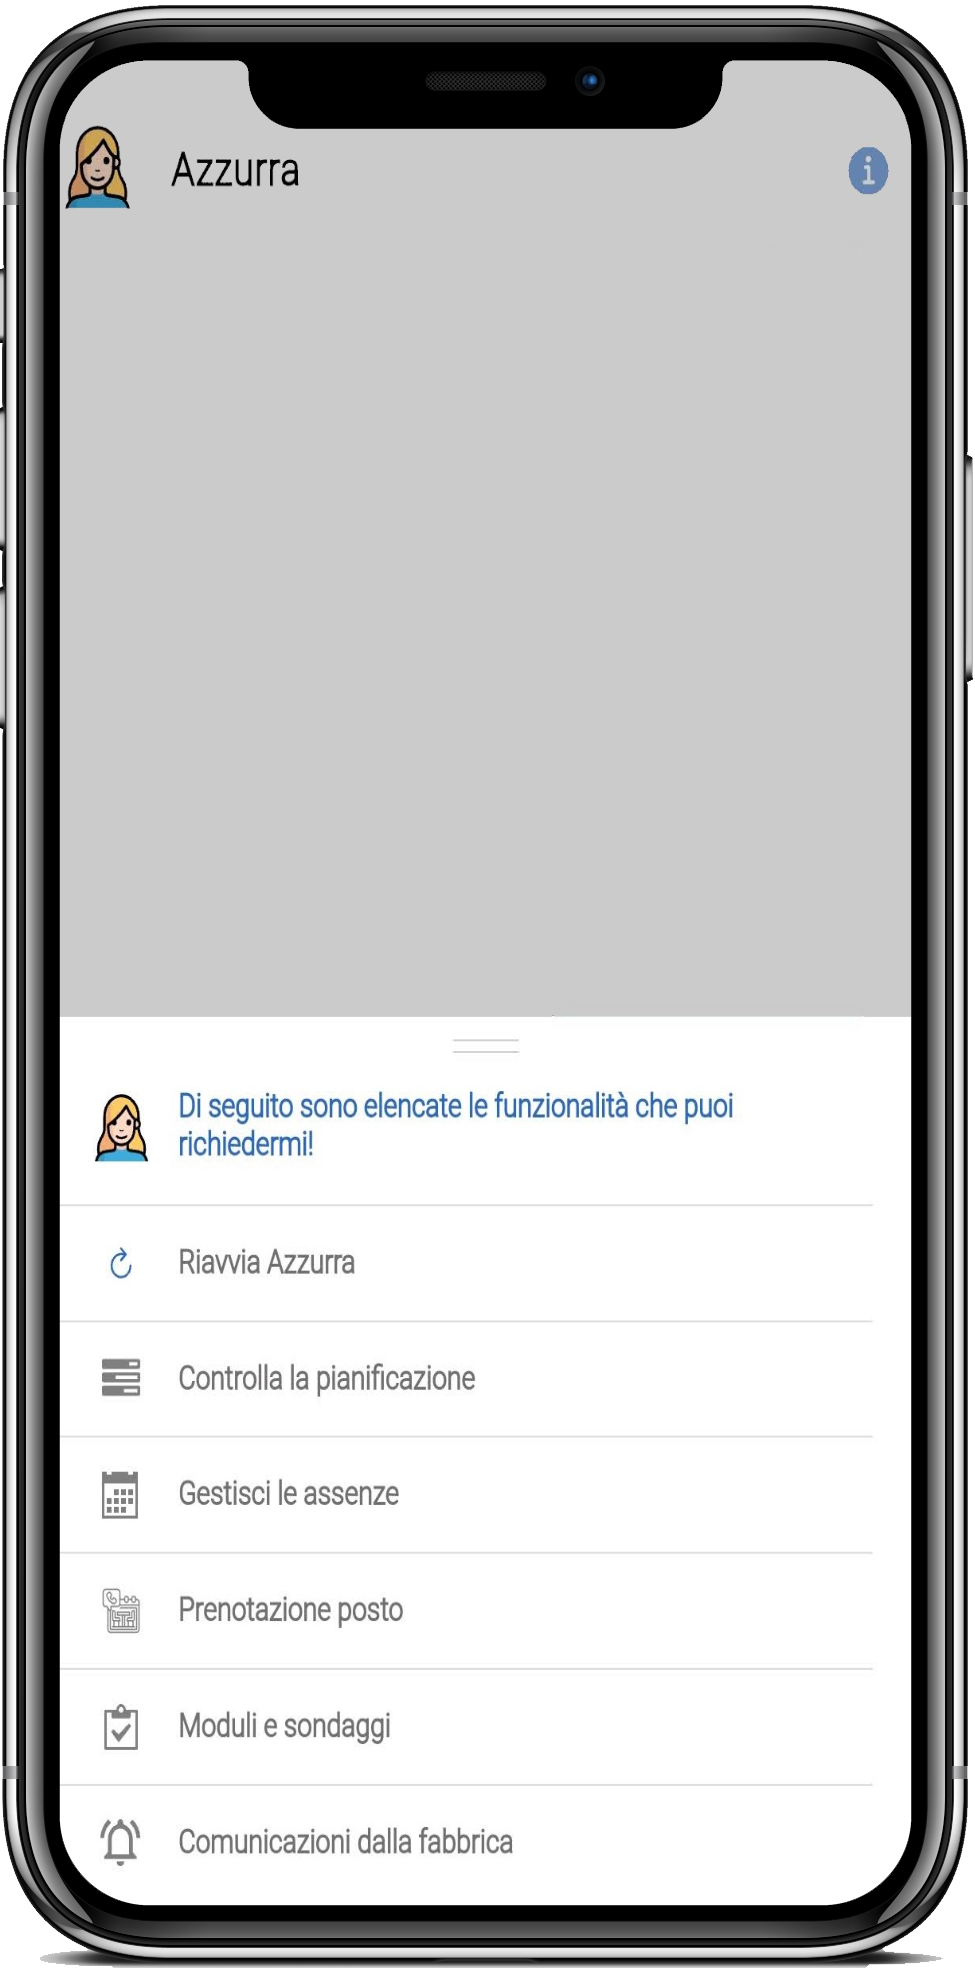
\includegraphics[scale=0.2]{shortcuts.png}
	\caption{Menu contenente le shortcuts disponibili}
\end{figure}

Il campo shortcuts viene indicato nel file con la \emph{keyword} shortcuts
e al suo interno contiene i seguenti campi:
\begin{itemize}
	\item text: È un campo che può essere di tipo \emph{string} e quindi contiene il testo da far visualizzare nel bottone della scorciatoia all'utente, oppure un oggetto che contiene un attributo per ogni lingua disponibile, dove ogni attributo ha il testo nella lingua straniera che l'attributo rappresenta. Il testo nella lingua di default (italiano) è contenuto nell’attributo “default” ;
	\item flowId: Contiene l'identificativo del flusso che la scorciatoia permette di far eseguire;
	\item icon: Per rendere la UI più accattivante è possibile aggiungere al bottone dedicato alla scorciatoia, delle icone per ogni scorciatoia.
\end{itemize}
\clearpage
\subsection{Configurazione "config"}
Il campo config permette di indicare attraverso il campo startBlockId quale blocco di conversazione del flusso deve essere eseguito per primo, per tale campo ci sarà il codice identificativo del primo blocco da eseguire. Il campo configurazione viene indicato nel file con la \emph{keyword} config.

\subsection{Blocchi per la conversazione "blocks"}
Il campo Blocchi indicato nel file con la \emph{keyword} blocks contiene tutti i blocchi per la conversazione i quali indicano i messaggi che devono essere mostrati e i passi da eseguire a seconda delle scelte inserite dell'utente umano.
I blocchi utilizzati per la conversazione si differenziano tra lo loro dal tipo di blocco a cui appartengono. Ogni tipo ha proprie caratteristiche uniche ma anche delle caratteristiche comuni, questo perché tutti i tipi di blocchi per la conversazione ereditano da un tipo padre detto BLOCK. I tipi figli di Block sono i seguenti:
\begin{itemize}
	\item\textbf{ASK};
	\item\textbf{SAY};
	\item\textbf{IF};
	\item\textbf{PROC};
	\item\textbf{JUMP};
	\item\textbf{CALLFUNC}.
\end{itemize}
Di seguito verrà illustrata la struttura e il ruolo di BLOCK e dei suoi figli.
\subsubsection{BLOCK}

BLOCK è il blocco di conversazione attraverso il quale tutti blocchi ereditano delle caratteristiche comuni della sua struttura, di fatto BLOCK non può essere utilizzato e, quindi, può essere paragonato a una classe astratta nell’ambito della programmazione ad oggetti, dove vengono definite delle caratteristiche della classe ma non può essere istanziata, perciò può essere solo ereditata dai suoi figli, che diventano classi concrete istanziabili.

%\begin{figure}[htbp]
%	\centering
%	\includegraphics[height=5cm]{img/block.png}
%	\caption{Definizione della classe BLOCK}
%\end{figure}

Ha la seguente struttura:

\begin{itemize}
	\item \textbf{id}: È un campo di tipo \emph{string} che identifica univocamente il blocco tra un insieme di blocchi di conversazione;
	\item \textbf{type}: Questo campo indica il tipo di blocco che come scritto può essere di tipo ASK
	 o SAY o IF o PROC o JUMP oppure CALLFUNC;        
	\item \textbf{text}: È un campo che può essere di tipo \emph{string} contente il testo da far visualizzare all'utente, oppure un oggetto che contiene un attributo per ogni lingua disponibile contente del testo nella corrispondente lingua, e un attributo default che contiene il testo di default;
	\item \textbf{variations}: Anch'esso è un tipo \emph{string} che contiene uno o più testi alternati al principale rappresentato dal campo text. Il funzionamento prevede che randomicamente il testo da mostrare all'utente non sarà quello principale ma uno delle alternative contenuto all'interno di variations, verrà perciò scelto in modo casuale, uno dei testi a disposizione; 
	\item \textbf{target}: Questo campo contiene l'id del prossimo blocco di conversazione da eseguire;
	\item \textbf{variable}: Questo campo indica il nome della variabile “conversazionale” su cui salvare eventuali valori di input inseriti dall’utente: il flow engine quindi, attraverso dei metodi specifici, ha la capacità di salvare tutte le scelte fatte dell’utente, memorizzandole nelle variabili indicate nel campo variable.
	\item \textbf{widget}: Indica il tipo di oggetto grafico detto Widget che deve essere utilizzato a supporto del blocco, esistono i seguenti tipi di Widget che verranno descritti successivamente:
	\begin{itemize}
		\item \textbf{BUTTONS};
		\item \textbf{ITEMS};
		\item \textbf{PICKER};
		\item \textbf{TIMEPICKER};
		\item \textbf{DATEPICKER};
		\item \textbf{CALENDAR};
		\item \textbf{QRSCANNER}.
	\end{itemize}
	\item \textbf{widgetOptions}:Permette di aggiungere delle opzioni in più al Widget, per esempio permette di indicare del testo all'interno dei Widget oppure indicare il valore minimo accettabile.
\end{itemize} 


\subsubsection{ASK}
Il blocco di conversazione ASK ha la funzione di mostrare all’utente una serie di opzioni disponibili e chiedere quali tra queste vuole eseguire. Quindi mostra le possibili scelte rimanendo in attesa di una risposta dell’utente. Infine esegue il comando collegato alla scelta effettuata dall’utente dirottando la conversazione al blocco successivo. 

\begin{figure}[htbp]
	\centering
	
\includegraphics[scale=0.25] {blockItems.jpg}
	\caption{Esempio di messaggio prodotto da un blocco di tipo ASK}
\end{figure}

Oltre a campi del tipo BLOCK ha i seguenti campi in più:

\begin{itemize}
	\item \textbf{category}: Il blocco ASK è ulteriormente distinguibile in ASK o in MENU che si differenziano nel seguente aspetto:\\
	nel caso sia di categoria ASK tutte le opzioni disponibili portano a un blocco di conversazione successivo diverso mentre per MENU tutte le opzioni portano tutte allo stesso blocco;
	\item \textbf{source}: Parametro che contiene il nome di una variabile a cui fare riferimento per prendere i dati da utilizzare. Se non si fa riferimento a nessuna variabile allora va settato a \emph{NULL};
	\item \textbf{items}: Questo campo contiene un array d'oggetti di tipo BlockItem che rappresentano le possibili scelte che può fare l'utente, essi graficamente vengono rappresentati come dei pulsanti;
	\item \textbf{sourceType}: Parametro che indica la modalità di utilizzo della variabile contenuta nel campo source;
	Sono previste due modalità:
	\begin{itemize}
		\item \textbf{LIST}: In questo caso la variabile contenuta in source viene ignorata e vengono presi tutti gli oggetti di tipo BlockItem contenuti nel campo items che vengono trasformati in bottoni da far visualizzare a video;
		\item \textbf{VARIABLE}: In questo caso tutto ciò che è contenuto nella variabile del campo source viene trasformato in bottoni da far visualizzare a video, per poterlo fare devono essere formattati in una struttura del tipo chiave valore.
	\end{itemize}	
\end{itemize} 

\subsubsection{SAY}

Il blocco di conversazione SAY ha la funzione di mostrare all'utente un messaggio a video attraverso il quale si comunica l'esito della operazione precedente e il risultato da essa ricavata. Perciò l'utente richiede l'esecuzione di una qualche operazione, viene eseguita e una volta conclusa il \gls{bot}\ap{[g]} risponderà all'utente con il risultato ricavato precedentemente.

\begin{figure}[htbp]
	\centering
	
\includegraphics[scale=0.25]{say.jpg}
	\caption{Esempio di messaggio prodotto da un blocco di tipo SAY}
\end{figure}
Oltre a campi del tipo BLOCK ha il seguente campo in più:

\begin{itemize}
	\item \textbf{attachments}: Campo che contiene un array d'oggetti di tipo BlockAttachment che permettono di allegare immagini o file PDF.
\end{itemize}

Inoltre sono presenti i campi items, source e sourceType, con analogo funzionamento del blocco ASK per inserire eventuali bottoni che aprono schede o link contenenti il risultato richiesto.

\subsubsection{IF}

Il blocco di conversazione IF ha la funzione di verificare se una o più condizioni sono rispettate. Perciò verifica se le condizioni sono soddisfatte, e in base all'esito verrà scelto il prossimo blocco da eseguire.

%\begin{figure}[htbp]
%	\centering
%	\includegraphics[scale=1]{img/if.png}
%	\caption{Definizione della classe IF}
%\end{figure}
Oltre a campi del tipo BLOCK ha i seguenti campi in più:

\begin{itemize}
	\item \textbf{conditions}: Contiene una o più condizioni che devono essere verificate;
	\item \textbf{trueBlockTarget}: Indica il blocco successivo da eseguire se le condizioni sono soddisfate;
	\item \textbf{falseBlockTarget}: Indica il blocco successivo da eseguire se le condizioni non sono soddisfate.
\end{itemize}


\subsubsection{PROC}
Il blocco di conversazione PROC permette di eseguire delle operazioni sulle variabili conversazionali cioè, assegnazione o trasformazione dei dati. Ad esempio, permette di riordinare i dati ricevuti dal server in modo da poter essere utilizzati dai source con sourceType uguale a VARIABLE.

%\begin{figure}[htbp]
%	\centering
%	\includegraphics[scale=1]{img/proc.png}
%	\caption{Definizione della classe PROC}
%\end{figure}

Oltre a campi del tipo BLOCK ha il seguente campo in più:

\begin{itemize}
	\item \textbf{expressions}: Contiene le espressioni da eseguire, ad esempio, per la formattazione dei dati.
	Ha i seguenti campi:
	\begin{itemize}
		\item \textbf{var}: Contiene il nome della variabile dove viene salvato il risultato della formattazione;
		\item \textbf{type}: Indica il tipo di formattazione che si vuole applicare, al momento c'è solo una formattazione disponibile:
		\begin{itemize}
			\item \textbf{reduce to textvalue}: Permette di riordinare i vari valori che si hanno in una struttura chiave valore.
		\end{itemize}
		\item \textbf{args}: Contiene un espressione in Handlebars, un linguaggio di \emph{templating} utilizzato per costruire \emph{template} in HTML con dei cosiddetti segnaposto che verranno poi valorizzati con dei valori, utilizzando delle \emph{keyword} del linguaggio, in modo da ottenere delle componenti in HTML da mostrare come messaggio.
	\end{itemize}
\end{itemize}

\subsubsection{JUMP}

Il blocco di conversazione JUMP permette di cambiare il flusso conversazionale ed eseguirne una altro. In termini tecnici si passa da un JSON di configurazione ad un altro dove ogni configurazioni in JSON contiene un specifico flusso di conversazione. Perciò, grazie a JUMP si può "saltare" da un flusso di conversazione a un altro.Il blocco di conversazione JUMP permette di cambiare il flusso conversazionale ed eseguirne un altro. In termini tecnici si passa da un JSON di configurazione ad un altro dove ogni configurazione in JSON contiene un specifico flusso di conversazione. Perciò, grazie a JUMP, si può "saltare" da un flusso di conversazione ad un altro.
Nel campo target in questo caso non viene indicato l’id del blocco successivo ma, l’id del \emph{flow} che si vuole eseguire.


%\begin{figure}[htbp]
%	\centering
%	\includegraphics[height=5cm]{img/jump.png}
%	\caption{Definizione della classe JUMP}
%\end{figure}


\subsubsection{CALLFUNC}

Il blocco di conversazione CALLFUNC è il blocco attraverso il quale, il \gls{bot}\ap{[g]} (l'applicazione mobile) può richiedere l’esecuzione di chiamate ad \gls{api}\ap{[g]} (interne o esterne). Attraverso un \gls{WebSocket}\ap{[g]}, che mantiene una connessione tra il \gls{bot}\ap{[g]} e Azzurra.io, quest’ultima richiama, a sua volta, delle \gls{api}\ap{[g]} di \gls{AWMS}\ap{[g]} (o esterne ad \gls{AWMS}\ap{[g]}) per ottenere i dati richiesti dell’utente o per salvare dati. 

%\begin{figure}[htbp]
%	\centering
%	\includegraphics[scale=1]{img/callfun.png}
%	\caption{Definizione della classe CALLFUNC}
%\end{figure}

Oltre a campi del tipo BLOCK ha il seguente campo in più:

\begin{itemize}
	\item \textbf{payload}: Campo che contiene l'intestazione e il corpo della richiesta verso Azzurra.io;
	Contiene i seguenti campi:
	\begin{itemize}
		\item \textbf{type}: Indica se la chiamata è verso Azzurra.io attraverso il valore \textsf{int} oppure verso un servizio esterno con il valore \textsf{ext}.
	\end{itemize}
	Se la chiamata è di tipo int ha la seguente struttura:
	\begin{itemize}
		\item \textbf{route}: Indica il metodo di Azzurra.io da richiamare;
		\item \textbf{body}: Contiene il corpo della richiesta, nello specifico un \emph{template} costruito da Handlebars che verrà idratato da Azzurra.io nel caso sia una richiesta di dati o dal \gls{bot}\ap{[g]} nel caso in cui debba inviare dei dati da salvare.
	\end{itemize}
	Se la chiamata è di tipo ext ha la seguente struttura:
	\begin{itemize}
		\item \textbf{config}: Contiene la struttura di una chiamata \gls{http}\ap{[g]}.\\
		Ha i seguenti campi:
		\begin{itemize}
			\item \textbf{url}: Contiene l'indirizzo URL del servizio esterno a cui fare richiesta;
			\item \textbf{method}: Se la richiesta e di tipo GET o POST;
			\item \textbf{headers}: Contiene l'intestazione per la richiesta HTTP;
			\item \textbf{params}: Contiene le variabili necessarie per la chiamata, questo campo viene usato solo se la richiesta e di tipo GET;
			\item \textbf{data}: Analogo al campo params solo se viene usato dai metodi POST.
		\end{itemize}
	\end{itemize}
	\item \textbf{var}: Indica il nome della variabile dove salvare il risultato della richiesta;
	\item \textbf{failureBlockTarget}: Indica il blocco successivo da eseguire se la richiesta non va a buon fine;
	\item \textbf{successBlockTarget}: Indica il blocco successivo da eseguire se la richiesta va a buon fine.
\end{itemize}

\subsection{Oggetti ausiliari}
Come scritto nella sezione precedente questi oggetti vengono definiti per essere utilizzati all’interno dei blocchi per svolgere un azione di supporto, affinché si possa raggiungere ciò per cui sono stati realizzati i blocchi di conversazione stessi.\\
Di seguito vengono indicate tutte le classi degli oggetti ausiliari disponibili.

\subsubsection*{Widget}
È un oggetto che a seconda del tipo permette di realizzare delle componenti grafiche, esso viene utilizzo per richiedere delle azioni da parte dell’utente umano.
Ha i seguenti tipi:
\begin{itemize}
	\item \textbf{BUTTONS}: Genera dei bottoni arrotondati;
	\begin{figure}[h]
		\centering
		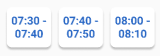
\includegraphics[scale=1.1]{buttons.png}
	\caption{Rappresentazione grafica dei buttons}
	\end{figure}
	\clearpage
	\item \textbf{ITEMS}: Genera dei bottoni quadrati;
	\begin{figure}[h]
		\centering
		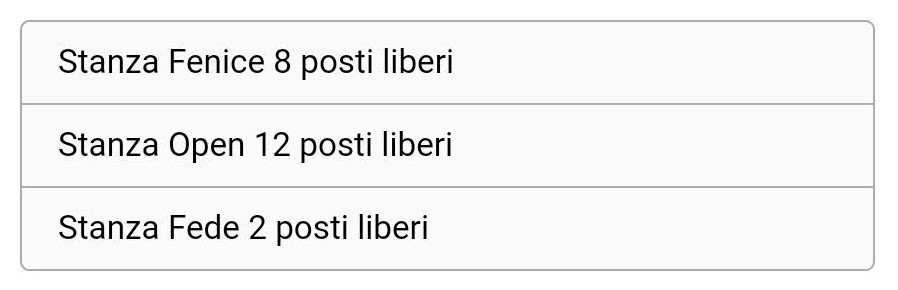
\includegraphics[scale=0.3]{items.jpg}
		\caption{Rappresentazione grafica degli items}
	\end{figure}
	\item \textbf{PICKER}: Genera, attraverso il componente “ion-picker” di \textsf{Ionic} una finestra di dialogo dove si può selezionare una opzione tra quelle proposte;
	\begin{figure}[h]
		\centering
		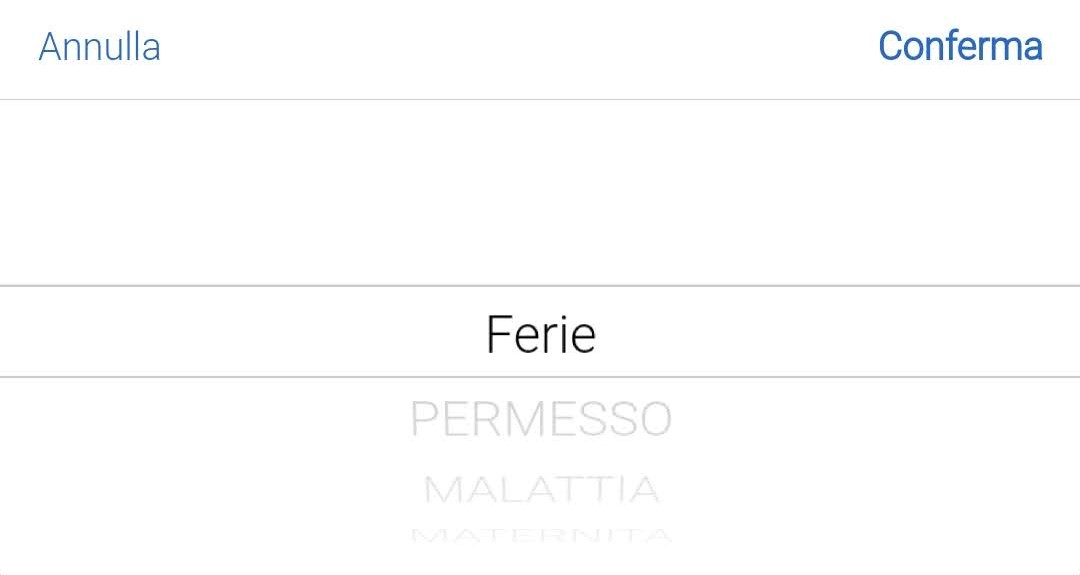
\includegraphics[scale=0.2]{picker.jpg}
		\caption{Rappresentazione grafica del picker}
	\end{figure}
	\item \textbf{TIMEPICKER}: Analogo al PICKER solo che le opzioni da scegliere è l'orario che si vuole selezionare;
	\begin{figure}[h]
		\centering
		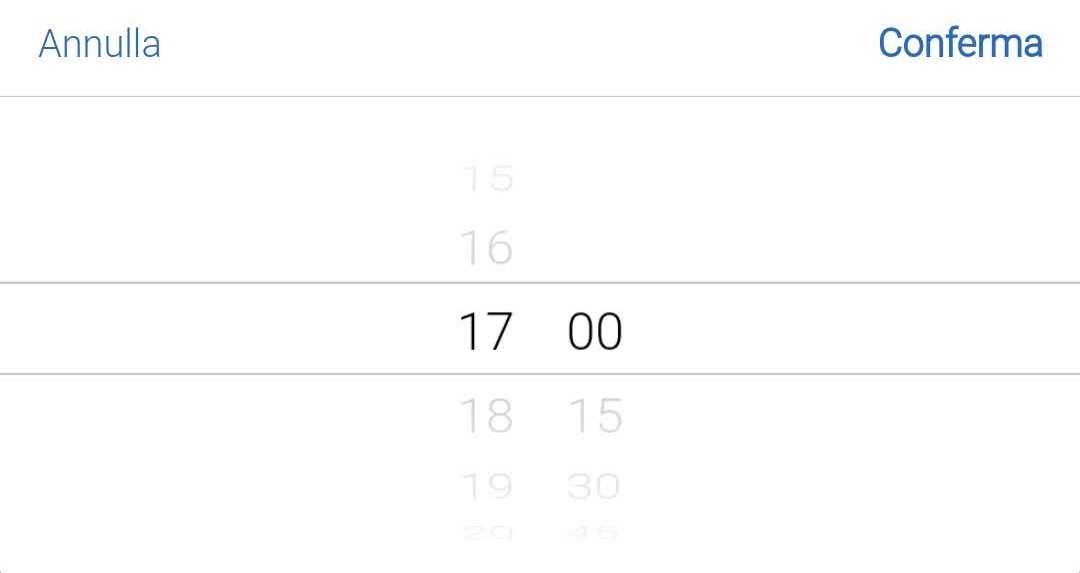
\includegraphics[scale=0.2]{timePicker.jpg}
		\caption{Rappresentazione grafica del time picker}\label{fig:time}
	\end{figure}
\clearpage
	\item \textbf{DATEPICKER}: Analogo al PICKER solo che le opzioni da scegliere è la data che si vuole selezionare;
	\begin{figure}[h]
		\centering
		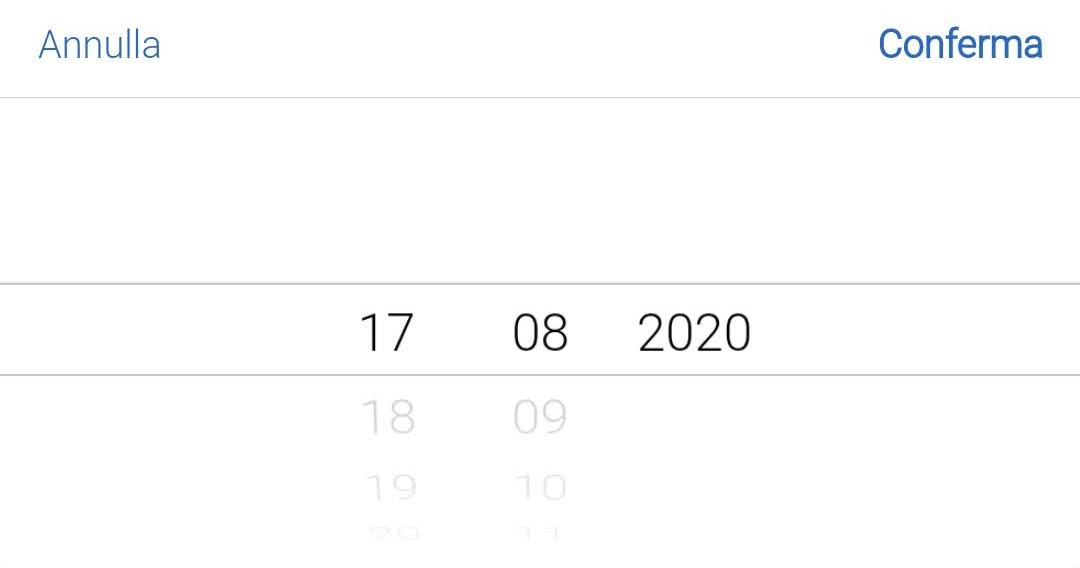
\includegraphics[scale=0.2]{datePicker.jpg}
		\caption{Rappresentazione grafica del date picker}\label{fig:date}
	\end{figure}
	\item \textbf{CALENDAR}: Fa comparire un calendario grazie all'utilizzo del plugin Calendar per Ionic;
	\item \textbf{QRSCANNER}: Permette di accedere alla fotocamera (solo se si hanno i permessi) e di decodificare i codici QR-code tutto ciò grazie al plugin QR Scanner di Cordova.
	\begin{figure}[h]
		\centering
		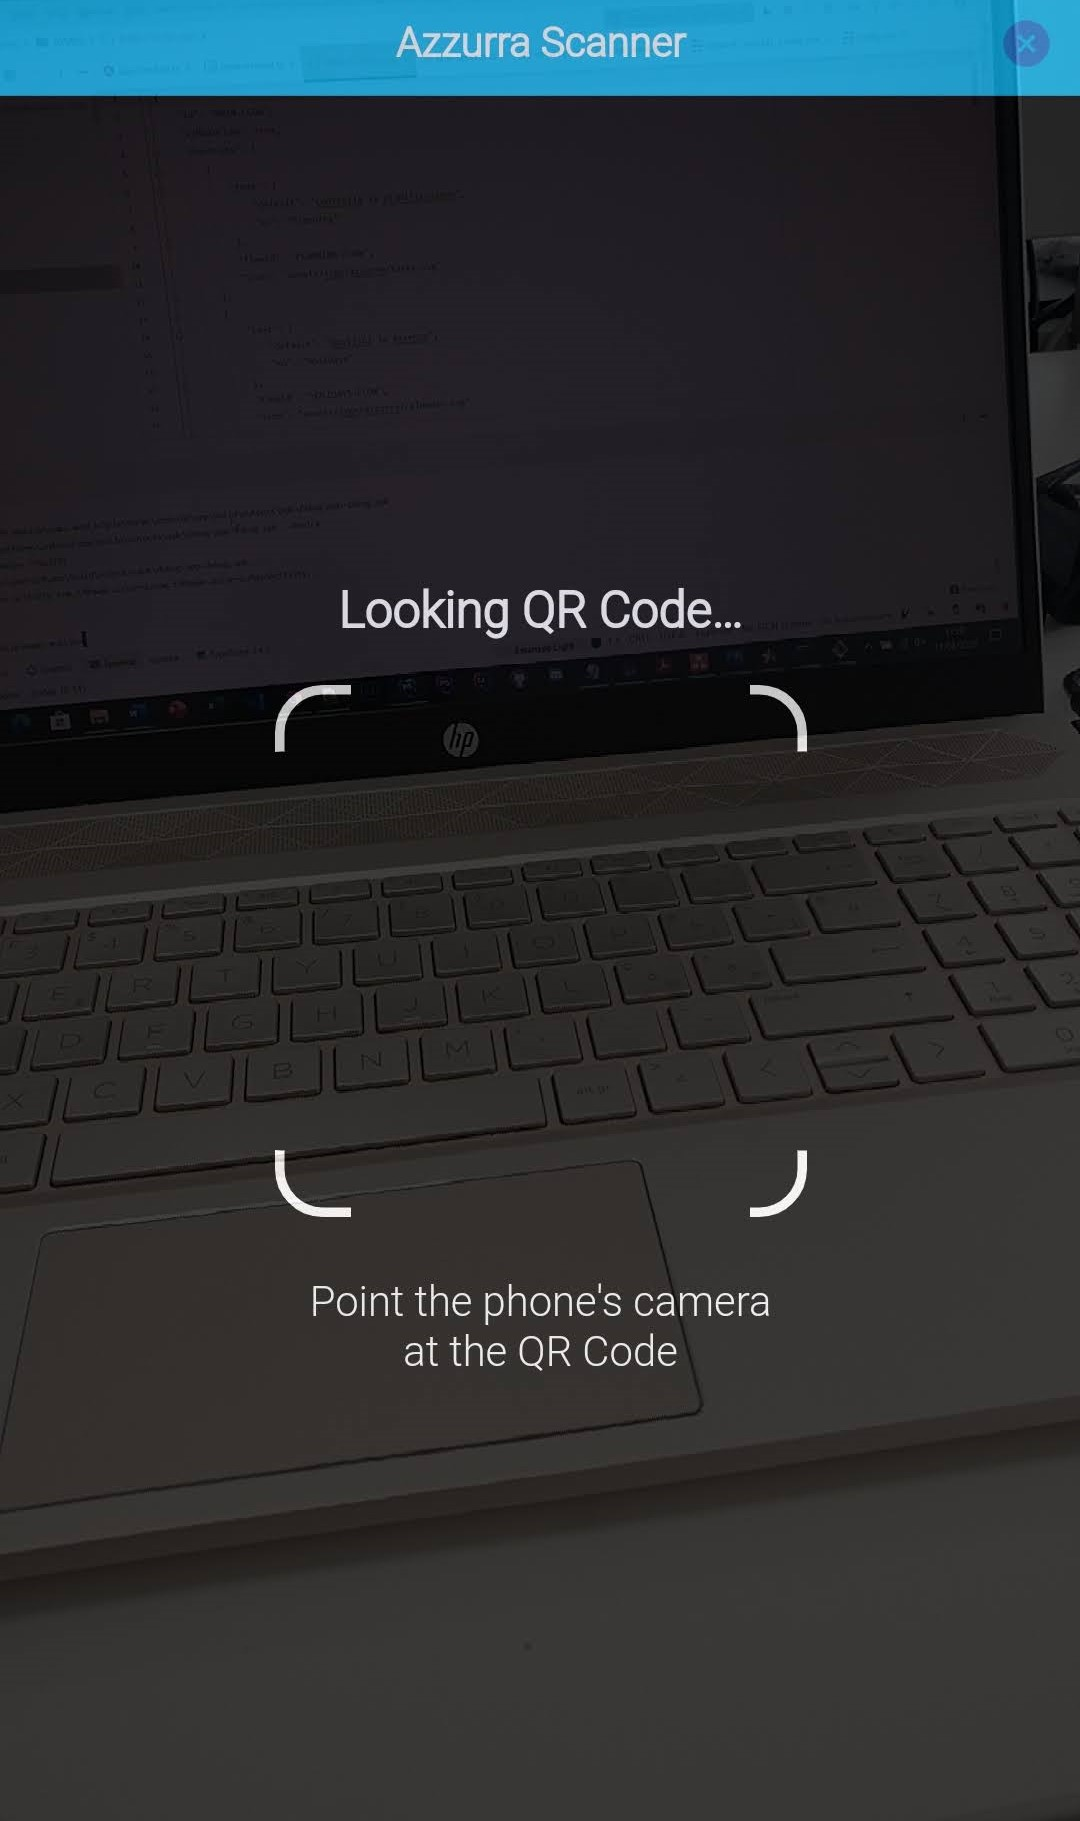
\includegraphics[scale=0.2]{qrcode.jpg}
		\caption{Rappresentazione grafica del QR scanner}\label{fig:qrc}
	\end{figure}
\end{itemize}

\subsubsection*{BlockItem}
Questo oggetto rappresenta una possibile scelta che può fare l'utente, graficamente viene rappresentato come un bottone cliccabile dall'utente.

\begin{figure}[h]
	\centering
	
\includegraphics[scale=0.3]{blockItems.jpg}
	\caption{Rappresentazione grafica del BlockItem}
\end{figure}
Ha la seguente struttura:

\begin{itemize}
	\item \textbf{text}: Contiene l'etichetta che viene visualizzata sul bottone;
	\item \textbf{target}: Contiene l'id del prossimo blocco da eseguire.
\end{itemize}



\subsubsection*{BlockAttachment} 
L'oggetto in esame permette di allegare immagini o file PDF da mostrare all'utente.

Ha la seguente struttura:

\begin{itemize}
	\item \textbf{id}: Contine un codice univoco che identifica ogni BlockAttachment;
	\item \textbf{type}: Indica se contiene un PDF o una immagine, nel caso di un'immagine indica se è in formato JPG o in JPEG oppure in PNG.
\end{itemize}	

\section{Gestione dell'internazionalizzazione di AWMS}
Per il sistema \gls{AWMS} è stata implementata la gestione dell'\gls{i18n}. Infatti per rendere tutto il sistema, sia lato backend sia lato Azzurra, adattabile a più lingue, sono stati definiti un insieme di testi multi-lingua. Per gestire questi testi multi-lingua è stato progettato di utilizzare un \emph{template engine} al fine di ottenere la parametrizzazione dei testi. \\

Un \emph{template engine} non è altro che un programma che prevede la definizione di blocchi detti \emph{template} spesso scritti in HTML, che hanno la caratteristica di avere dei segnaposto detti \emph{placeholders}, che vengono sostituiti dai dati da visualizzare. In questi blocchi perciò  viene definito il testo scritto in una specifica lingua e in quali punti del testo devono essere inseriti i dati per la visualizzazione. Per la sostituzione dei \emph{placeholders} solitamente il \emph{template engine} utilizza file \gls{JSON}\ap{[g]}, in cui i segnaposti sono solitamente rappresentati dai campi che compongono l’oggetto salvato nel file JSON, i quali andranno a sostituire i segnaposti con i loro valori che rappresentano i dati da visualizzare. Chiaramente i \emph{template} vengono riutilizzanti anche se i dati visualizzati variano. Vengono perciò definiti \emph{template} di testi "localizzati" cioè scritti in un delle lingue supportate dal sistema \gls{AWMS}.\\

 Un \emph{template engine} può essere facilmente implementato in JavaScript ma come scelta progettuale di è stato deciso di utilizzare \emph{Handlebars}. \emph{Handlebars} è un estensione del \emph{template engine} \emph{mustache} perché, per indicare i \emph{placehorders} all'interno dei \emph{template} utilizza le doppie parentesi graffe le quali racchiudono la parola da sostituire. È stato scelto di utilizzare \emph{Handlebars} perché garantisce delle performance migliori infatti, permette di compilare i \emph{template}, riducendo il tempo di \emph{rendering} quando un blocco di codice viene creato più di una volta. Inoltre \emph{Handlebars} permette di utilizzare i cosiddetti "Helpers" che permettono l'esecuzione di funzionalità che vanno a manipolare la formattazione del testo. Infine, un’altra caratteristica avanzata di \emph{Handlebars} è il supporto ai "Partials". Con tale termine si indica la possibilità di innestare \emph{template} l’uno dentro l’altro, permettendone la riusabilità e la realizzazione di codice più ordinato.\\
 
 Nel lato backend ciascun testo "localizzato" è persistito in apposite tabelle di un \emph{database}.\\
 
 Nel lato \gls{bot}\ap{[g]} Azzurra come spiegato in precedenza, nel campo text dei blocchi conversazionali, c'è un oggetto che contiene un attributo per ogni lingua disponibile contente del testo nella corrispondente lingua, e un attributo default che contiene il testo di default. Quindi Il flow engine, interpretando ciascun blocco conversazionale, effettua un processamento dei testi scegliendo, se presenti, quelli relativi alla lingua dell'utente.\\
 
 Sara poi compito di \emph{Handlebars} "idratare" i \emph{template} cioè,  sostituiti, se presenti, i \emph{placeholders} in sintassi \emph{mustache} con dati da visualizzare.\\

 Durante lo stage un parte del tempo è stata dedicata allo studio di \emph{Handlebars} e alla scrittura dei \emph{template} che in molti casi, richiedevano l'inserimento dei \emph{placeholders} con la sintassi \emph{mustache}.
 

\section{Funzionamento di Azzurra Flow Engine}
L'Azzurra Flow Engine è l'elemento in grado di interpretare i dati contenuti nelle configurazioni JSON. Grazie a esso è possibile eseguire il corretto flusso della conversazione e generare i messaggi da mostrare nella \emph{chat} dell'applicazione mobile. 
\subsection{Messaggio del bot Azzurra}
Per implementare le funzionalità del Azzura Flow Engine vengono utilizzate le seguenti classi sviluppate in Angular:
\begin{itemize}
	\item \textbf{FlowService}: Ha i metodi necessari per interpretare le configurazioni JSON e quindi, per poter sapere quale tipo di messaggio deve essere costruito, ricavare i dati necessari per costruire i messaggi e sapere come procedere con la conversazione;
	\item \textbf{AzzurraService}: Permette principalmente di fare da tramite tra il FlowService e il \textbf{ChatComponent} per la creazione della conversazione. Oltre a ciò permette di gestire operazioni ad alto livello come il caricamento dei messaggi precedenti nella \emph{chat} e gestire le notifiche che possono arrivare dalla \emph{dashboard};
	\item \textbf{ChatComponent}: Si occupa di far visualizzare i messaggi della conversazione;
	\item \textbf{ChatService}: Ha il compito di creare e gestire i Widget da aggiungere al messaggio da mostrare, e inoltre, di ricavarne da essi le risposte dell'utente umano.
\end{itemize}

\begin{figure}[htbp]
	\centering
	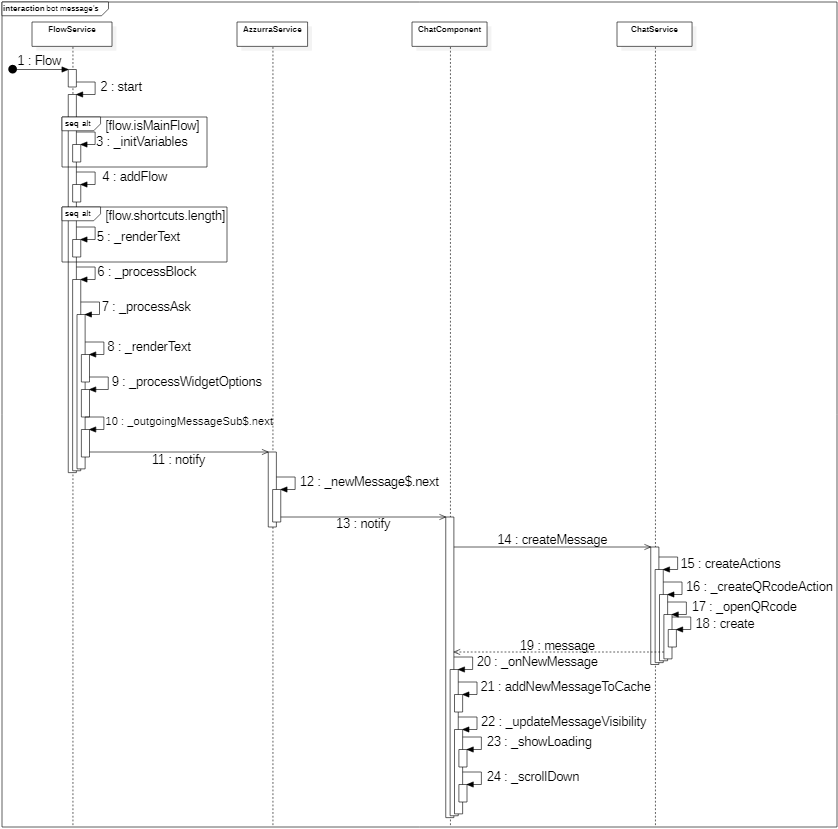
\includegraphics[height=20cm, width=14cm]{sd_bot_mx2.png}
	\caption{Diagramma di sequenza del processo di generazione del messaggio del bot Azzurra}\label{fig:mxBot}
\end{figure}

Una volta che si è stabilità la connessione con Azzurra.io, attraverso un \gls{WebSocket}\ap{[g]}, inizializzato il Flow Engine e infine, ricevuto la configurazione JSON contenente il flusso conversazionale, la generazione di un messaggio da parte del \gls{bot}\ap{[g]} Azzurra prevede i seguenti passi:\\
\begin{enumerate}
	\item Viene inviato all’applicazione mobile il flusso conversazionale richiesto precedentemente;
	\item Viene avviato nel FlowService il metodo start(), il quale riceve in input il flusso da eseguire. Viene verificato se il flusso ricevuto risulta essere il \emph{main flow}, in questo caso vengono inizializzate le variabili conversazionali d'ambiente utilizzate come supporto per la generazione dei messaggi, ad esempio esiste una variabile d'ambiente per indicare il giorno corrente o il formato della data da utilizzare;
	\item Una volta impostate le variabili conversazionali d’ambiente e usciti dal blocco condizionale viene salvato il flow da eseguire attraverso il metodo \_addFlow() che imposta come flusso corrente da eseguire il flusso ricevuto in input. Viene infine controllato se la configurazione definisce delle eventuali shortcuts;
	\item Se ci sono delle shortcuts viene chiamato il metodo \_renderText() per crearle, esso sarà in grado di interpretare il pezzo di configurazione dove sono definite le proprietà di ogni shortcuts;
	
	Una volta finita l'esecuzione del metodo, l'esecuzione torna al metodo start().
	\item Sempre in start() viene chiamata l'esecuzione di \_processBlock() dandogli in input il primo blocco del flusso da eseguire
	
	\item Nel metodo \_processBlock() viene eseguito il blocco che riceve in input, in questo caso il blocco da eseguire è il primo blocco del flusso come detto nel punto precedente. In questo metodo si verifica innanzitutto se c'è un blocco da eseguire, se non c'è viene emesso un segnale che informa che il flusso di conversazione è terminato, mentre se c'è un blocco allora si imposta questo blocco come quello in esecuzione e si verifica di che tipo è il blocco.\\
	A seconda del tipo del blocco vengono eseguite le seguenti istruzioni:
	\begin{itemize}
		\item \textbf{Caso SAY}: Viene eseguito il metodo \_processSay() ricevendo in input il blocco corrente. Il metodo prende il valore salvato nel campo text e le eventuali variations del blocco, generando il testo del messaggio da mostrare attraverso il metodo \_renderText(). Vengono generati eventuali BlockItems attraverso il metodo \_buildSayItems() il quale controlla il sourceType e in base al valore che ha, genera i BlockItems. Tornando in \_processSay(), se presenti vengono anche eseguite le widgetOptions attraverso il metodo \_processWidgetOptions() e creati gli eventuali BlockAttachments. Infine, viene emesso il nuovo messaggio creato per il \gls{bot}\ap{[g]} Azzurra e si passa all'esecuzione del prossimo blocco;
		\item \textbf{Caso ASK}: Viene eseguito il metodo \_processAsk ricevendo in input il blocco corrente. Il metodo salva il nome della variabile contenuta nel campo var, che contiene la risposta dell'utente. Analogamente per quanto accede per il blocco SAY viene creato il testo della domanda e attraverso il metodo \_buildQuestions() vengono creati i BlockItems delle possibili scelte. Inoltre, vengono processati gli eventuali widgetOptions. Infine, viene emesso il nuovo messaggio creato per il bot, il quale rimane in attesa della risposta dell'utente umano quando verrà visualizzato il messaggio;
		\item \textbf{Caso JUMP}: Viene eseguito il metodo \_processJump() ricevendo in input il blocco corrente. Richiama il metodo \_getFlow() pasandogli l'identificativo del flusso da eseguire attraverso il campo target. Il metodo citato richiede ad Azzurra.io il flusso che ha l'identificativo uguale a quello ricevuto in input, e una volta ricevuto comincia l'esecuzione del nuovo flusso conversazionale richiamando start();
		\item \textbf{Caso IF}: Viene eseguito il metodo \_processIf() passando in input il blocco corrente. Valuta la condizione attraverso \_manageConditions(), e in base al risultato stabilisce quale sarà il blocco di conversazione successivo da eseguire;
		\item \textbf{Caso PROD}: Viene eseguito il metodo \_processProd() passandogli in input il blocco corrente. Stabilisce che formattazione deve essere fatta e la esegue attraverso il metodo \_manageExpressions(). Infine, passa all'esecuzione del prossimo blocco;
		\item \textbf{CALLFUNC}: Viene ricavato il \emph{payload} del blocco e codificato il \emph{template} in Handlebars per generare il corpo della richiesta, una volta fatto ciò la richiesta è pronta e viene mandata a Azzurra.io. Successivamente viene salvata la risposta sulla variabile indicata del campo var e in base alla risposta, se andata a buon fine oppure no, si eseguirà il corrispondente blocco successivo.
	\end{itemize}	
	\item Nella Figura~\ref{fig:mxBot} viene mostrato il caso in cui viene eseguito il metodo \_processAsk() perché il blocco attuale e di tipo ASK;
	\item Viene eseguito \_renderText() per costruire il testo della domanda;
	\item Attraverso \_buildQuestions() vengono creati i BlockItems delle possibili scelte;
	\item Viene eseguito il metodo \_processWidgetOptions() per creare le eventuali widgetOptions;
	\item A questo punto la struttura del messaggio è stata creata, manca solo la visualizzazione nella \emph{chat} che è compito di ChatComponent, perciò attraverso il metodo next() di Angular, viene emesso un segnale che avvisa chi è in ascolto su \_outgoingMessageSub\$ che è stato creato un nuovo messaggio e che occorre visualizzarlo;
	\item Viene notificato agli ascoltatori l'evento descritto al punto precedente;
	\item Nel AzzuraService c'è un ascoltatore che riceve i segnali mandati dai metodi di FlowService, perciò con la notifica inviata al punto precedente AzzuraService ha il messaggio che è stato appena creato;
	\item AzzuraService emettere a sua volta il nuovo messaggio appena ricevuto, verso l'ascoltatore presente in ChatComponent;
	\item Quando ChatComponent riceve il messaggio eseguirà il metodo createMessage() di ChatService passandogli il messaggio ricevuto. Questo metodo si occuperà di far creare il messaggio grafico nel modo corretto.
	Innanzitutto, verifica chi ha emesso il messaggio, se è stato l'utente umano o il \gls{bot}\ap{[g]} Azzurra. Nel caso in cui il messaggio sia del \gls{bot}\ap{[g]} Azzurra viene indicato il testo da mostrare estraendolo dal messaggio ricevuto in input e aggiunto lo sprite di Azzurra per indicare graficamente che il messaggio viene dal bot;
	\item Nel caso in cui il messaggio preveda delle azioni da parte dell'utente umano, ovvero ci siano dei Widget, viene chiamato il metodo createAction() passandogli sempre il messaggio. In questo metodo viene verificato che tipo di Widget deve essere creato, per ogni Widget c'è un corrispondente metodo che ne imposta il testo da far visualizzare quando l'utente interagisce con esso, tale testo potrebbe essere un testo di default o un testo indicato nel campo widgetOptions inoltre nel caso del DATEPICKER o TIMEPICKER, viene impostato il formato di visualizzazione del giorno e dell'ora;
	\item Nel caso rappresentato dalla Figura~\ref{fig:mxBot}, viene chiamato il metodo \_createQRcodeAction()
	 il quale imposta il testo da mostrare e chiama il metodo \_openQRcode();
	\item \_openQRcode() Richiama il metodo create() per creare e aprire il Widget QRCODE;
	\item In \_openQRcode() viene chiamato il metodo create() che permette di utilizzare il ModalController di Ionic il quale crea una nuova finestra grafica con dentro la classe che gestisce il lettore di \gls{QR code}\ap{[g]}. Si crea quindi graficamente il Widget. I corrispondenti metodi \emph{open} per DATEPICKER e TIMEPICKER non utilizzano il ModalController ma utilizzano una componente grafica messa a disposizione da Ionic, perciò in questi metodi viene configurato il componente grafico senza richiamare nessuna classe;
	\item Terminata la creazione il messaggio viene ritornato il messaggio costruito a ChatComponent;
	\item Con onNewMessage() viene inserito nella \emph{chat} il nuovo messaggio;
	\item Il nuovo messaggio viene inviato a Azzurra.io, per essere memorizzato, attraverso il metodo addNewMessageToCache();
	\item Viene aggiornata la \emph{chat} per mostrare il nuovo messaggio con il metodo \_updateMessageVisibility();
	\item \_updateMessageVisibility() chiama \_showLoading() per simulare un caricamento;
	\item Infine, \_updateMessageVisibility() chiama \_scrollDown() per muovere verso il basso la \emph{chat} in modo da mostrare il nuovo messaggio che altrimenti rimarrebbe nascosto.
\end{enumerate}

Una volta che l'utente interagisce con il Widget deve essere creato il messaggio dell'utente umano con la sua risposta. 
\clearpage
\subsection{Messaggio dell’utente  umano}
La generazione di un messaggio da parte dell’utente umano prevede le seguenti azioni:\\
\begin{figure}[htbp]
	\centering
	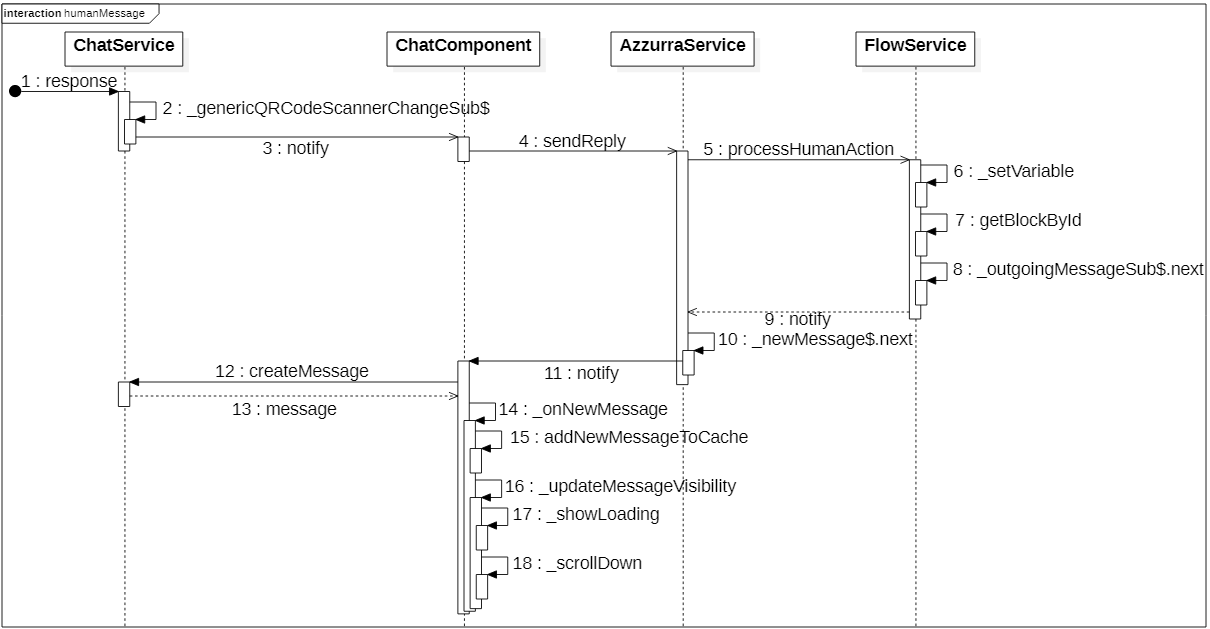
\includegraphics[height=11cm, width=13cm]{sd_human_mx.png}
	\caption{Diagramma di sequenza del processo di generazione del messaggio del bot Azzurra}\label{fig:mxHuman}
\end{figure}
\begin{enumerate}
	\item Quando l'utente esegue un'azione che genera una risposta da parte sua, il ChatService emette il valore della risposta ogni volta che un Widget la riceve;
	\item Nel ChatComponent esiste un ascoltatore per ogni evento emesso da ogni Widget. Nella Figura~\ref{fig:mxHuman} viene rappresentato il caso in cui il Widget sia di tipo QRCODE perciò, attraverso il metodo next() di Angular, viene emesso un segnale che avvisa a chi e in ascolto su  \_genericQRCodeScannerChangeSub\$ che è stato emesso un evento da QRCODE inserendo anche il valore letto dallo scanner;
	\item Viene notificato agli ascoltatori l'evento descritto al punto precedente;
	\item ChatComponent riceve la notifica e chiama il metodo sendReply() di AzzurraService dandogli in input il valore letto dallo scanner ricevuto dalla notifica solo se il messaggio è valido, se non lo è viene ignorato;	
	\item Il metodo sendReply() chiama a sua volta processHumanAction() di FlowService;
	\item In processHumanAction() viene creata la struttura del messaggio con la risposta dell'utente perciò, viene richiamato il metodo \_setVariable() in cui, viene impostato il valore della risposta ritornato dal Widget che è stato salvato nella variabile indicata nel campo var;
	\item In processHumanAction() viene richiamato il metodo getBlockId() che verifica se il Widget abbia al suo interno un proprio campo target, se sì viene impostato come prossimo blocco di conversazione il blocco che ha il codice identificativo uguale a quello contenuto nel target, se invece non ha un campo target proprio si va a prendere il valore del campo target del blocco e si imposta il suo valore come prossimo blocco da eseguire;
	\item Attraverso il metodo next() di Angular, viene emesso un segnale che avvisa a chi e in ascolto su \_outgoingMessageSub\$ che è stato emesso un nuovo messaggio;
	\item Viene notificato agli ascoltatori l'evento descritto al punto precedente;
	\item AzzurraService riceve la notifica e tramite il metodo next() avvisa e invia la struttura del nuovo messaggio a tutti coloro che sono in ascolto su \_newMessage\$;
	\item Viene notificato agli ascoltatori l'evento descritto al punto precedente;
	\item ChatComponent riceve il messaggio e chiama il metodo createMessage() di ChatService passandogli il messaggio ricevuto. Questo metodo si occuperà di far creare il messaggio grafico nel modo corretto. In questo caso il messaggio e di tipo umano perciò verrà creato secondo una certa specifica;
	\item Viene ritornato il messaggio a ChatComponent;
	\item Infine, per visualizzare il messaggio sulla \emph{chat}, vengono rifatte le stesse operazioni che erano state fatte per il messaggio del \gls{bot}\ap{[g]} Azzurra.
\end{enumerate}

